\documentclass{standalone}
% translate with >> pdflatex -shell-escape <file>

% This file is an extract of the PGFPLOTS manual, copyright by Christian Feuersaenger.
% 
% Feel free to use it as long as you cite the pgfplots manual properly.
%
% See
%   http://pgfplots.sourceforge.net/pgfplots.pdf
% for the complete manual.
%
% Any required input files (for <plot table> or <plot file> or the table package) can be downloaded
% at
% http://www.ctan.org/tex-archive/graphics/pgf/contrib/pgfplots/doc/latex/
% and
% http://www.ctan.org/tex-archive/graphics/pgf/contrib/pgfplots/doc/latex/plotdata/

\usepackage{pgfplots}
\usepackage{pgfplotstable}
\pgfplotsset{compat=newest}

% The manual loads these libraries globally; the extracted standalone examples
% need them too. external/clickable/snakes are intentionally omitted.
\usetikzlibrary{
	arrows.meta,backgrounds,calc,decorations.footprints,decorations.markings,
	decorations.pathreplacing,fixedpointarithmetic,intersections,patterns,
	plotmarks,shapes.arrows,spy,through}
\usepgfplotslibrary{
	colorbrewer,colormaps,dateplot,fillbetween,groupplots,patchplots,polar,
	smithchart,statistics,ternary,units}

% Some colormap examples reuse this display style defined earlier in the manual.
\pgfplotsset{
	cycle from colormap manual style/.style={
		x=3cm,y=10pt,ytick=\empty,
		colorbar style={x=,y=,ytick=\empty},
		point meta min=0,point meta max=1,
		stack plots=y,
		y dir=reverse,colorbar style={y dir=reverse},
		every axis plot/.style={line width=2pt},
		legend entries={0,...,20},
		legend pos=outer north east,
	},
}

\pagestyle{empty}

\usepgfplotslibrary{ternary}
\usepackage{textcomp}

\begin{document}
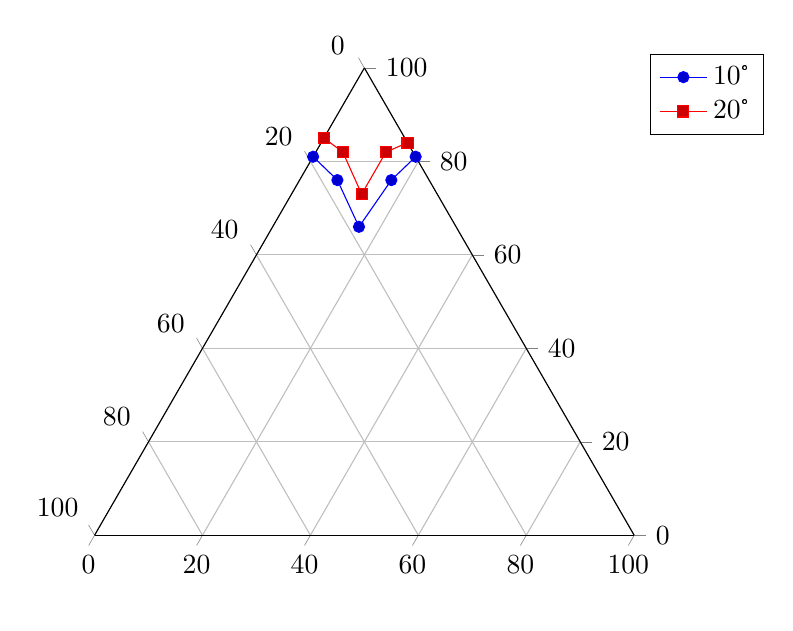
\begin{tikzpicture}
\begin{ternaryaxis}
    \addplot3 coordinates {
        (0.81,    0.19,    0.00)
        (0.76,    0.17,    0.07)
        (0.66,    0.16,    0.16)
        (0.76,    0.07,    0.17)
        (0.81,    0.00,    0.19)
    };

    \addplot3 coordinates {
        (0.85,    0.15,    0.00)
        (0.82,    0.13,    0.05)
        (0.73,    0.14,    0.13)
        (0.82,    0.06,    0.13)
        (0.84,    0.00,    0.16)
    };
    \legend{$10$\textdegree, $20$\textdegree}
\end{ternaryaxis}
\end{tikzpicture}
\end{document}
